%\documentclass[a4paper,english,12pt,twocolumn]{article}
\documentclass[a4paper,english,12pt]{article}
\usepackage[utf8]{inputenc} % Encodage du fichier
\usepackage[T1]{fontenc} % Encodage des fonts nécessaire pour le Latin
\usepackage[french]{babel} % Pour changer la langue des mots générés et choisir la bonne mise en page
\usepackage{amssymb}
\usepackage{pdflscape}
\usepackage{microtype} 
\usepackage{lmodern} % Le latin modèrne
\usepackage[top=2cm, bottom=2cm, left=2.5cm, right=1.5cm]{geometry} % Définir les marges de la page 
\usepackage[hidelinks,urlcolor=blue,unicode=true,
pdftitle={Twitter sentiment analysis},
pdfauthor={BELOUADAH Eden and BOUHAHA Mariem},
pdfdisplaydoctitle=true]{hyperref} % Pour les liens 
\usepackage{fancyhdr} % Pour le style de la page
\usepackage[font=it]{caption} % Rendre les titres des tableaux italiques
\usepackage{graphicx} % Pour les images
\usepackage{subcaption} % Pour mettre plusieurs images sur la même ligne
\usepackage{float} % Pour empêcher le déplacement des tableaux et des figures.
\usepackage{babelbib} % Pour changer la langue dans la bibliographie
\usepackage{amsmath} % Pour des fonctions mathématiques
\usepackage{amssymb} % Pour les symboles mathématiques
%\usepackage[onelanguage,english,longend,boxruled,algoruled,linesnumbered,algochapter,nofillcomment]{algorithm2e} %pour les algorithmes
\usepackage{multirow}
\usepackage{booktabs}
\usepackage{enumitem}
\usepackage{setspace}
\usepackage{longtable}
\graphicspath{ {images/} } 

\DisableLigatures[f]{encoding=*}

%Active ça si tu ne veux pas les points-virgules dans les algorithmes
% \DontPrintSemicolon
 
%\renewcommand \thechapter{\Roman{chapter}} % Utiliser les numéros romans pour les chapitres

\captionsetup{labelfont=it,textfont=it,labelsep=period} % Changer le style des légendes
\AtBeginDocument{ % Changer les légendes
	\renewcommand\tablename{\itshape Tableau}
	\renewcommand{\figurename}{\itshape Figure}
	% Renommer la table des matières
	\renewcommand{\contentsname}{Sommaire}
}

% Style de l'entête et le pied de la page
\setlength{\headheight}{16pt}
\pagestyle{fancy}
\fancyhead[L]{} % Enlever la section
\fancyhead[R]{\footnotesize\slshape{\nouppercase{\leftmark}}} % Titre du chapitre en minuscule avec taille 10
\fancyfoot[C]{}
\fancyfoot[R]{\thepage} % Déplacer le numéro de la page vers la droite de la page

\fancypagestyle{plain}{
\renewcommand{\headrulewidth}{0pt}
\fancyhf{}
\fancyfoot[R]{\thepage}
}
  
% Espace entre les lignes
\linespread{1.3}

% Code pris de https://tex.stackexchange.com/a/95616/109916 et corrigé
% Début
\makeatletter
\newcommand{\emptypage}[1]{
  \cleardoublepage
  \begingroup
  \let\ps@plain\ps@empty
  \pagestyle{empty}
  #1
  \cleardoublepage
  \endgroup}
\makeatletter
% Fin


% pour changer les deux points des légendes d'algorithmes
% \SetAlgoCaptionSeparator{\unskip.}

\begin{document}
%\include{Page_de_garde}
%\include{Remerciements}
\emptypage{
%\tableofcontents
%\listoffigures
%\listoftables
}
    
\setlength{\parskip}{0.6em plus 0.1em minus 0.1em}
%\SetKwInput{KwOut}{Outpits}

% Redéfinition des chapitres et sections pour les inclure dans le sommaire
\makeatletter
%	\let\oldchapter\chapter
%	\newcommand{\@chapterstar}[1]{\cleardoublepage\phantomsection\addcontentsline{toc}{chapter}{#1}{\oldchapter*{#1}}\markboth{#1}{}}
%	\newcommand{\@chapternostar}[1]{{\oldchapter{#1}}}
%	\renewcommand{\chapter}{\@ifstar{\@chapterstar}{\@chapternostar}}
\let\oldsection\section
\newcommand{\@sectionstar}[1]{\phantomsection\addcontentsline{toc}{section}{#1}{\oldsection*{#1}}}
\newcommand{\@sectionnostar}[1]{{\oldsection{#1}}}
\renewcommand\section{\@ifstar{\@sectionstar}{\@sectionnostar}}	
\newcommand*{\rom}[1]{\expandafter\@slowromancap\romannumeral #1@}
\makeatother

\setcounter{page}{1}
%%%%%%%%%%%%%%%%%%%%%%%%%%%%%%%%%%%%%%%%%%%%%%%%%%%%%%%%%%%%%

\title{Twitter Sentiment Analysis: A comparative approach}

\author{Mariem BOUHAHA \and Eden BELOUADAH}
% \date{}
\maketitle



\section{Introduction}
Text classification is a class of problems that finds application in many tasks, mainly sentiment analysis, predicting movie reviews as well as classifying emails as spam or not.

In recent literature, deep learning seems to be promising for text classification, achieving state-of-the-art results on a suite of standard  benchmark problems. 

In this project, we aim to compare and analyze the performance of several deep architectures that we use for sentiment analysis from tweets. For that, we studied the behavior of some deep neural networks as well as the influence of data representation on the models' performances. 

In this intermediate report, we will present the data in hand as well as some statistics to describe it, then we will give a brief description of the models tested so far and finally present the preliminary results. 

\section{Presenting the data}
For this project, we used the B-task SemEval-2013 [1] training and test data, which have the following characteristics before any preprocessing:

\begin{table}[H]\centering
\begin{tabular}{|c|c|c|c|c|}

\hline
Set & Number of examples & Positive & Negative & Neutral\\
\hline
Train & 5916 & 2179 & 816 & 2921\\
\hline
Test & 876 & 324 & 158 & 394\\
\hline

\end{tabular}
\caption{Classes distribution for train set and test set}
\end{table}

If we visualize an extract (the first 5 for example) of the tweets in the training set, we get the text shown in figure \ref{extract}.

\begin{figure}[h!]
\centering
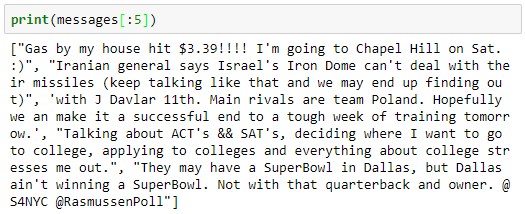
\includegraphics[scale=1]{extract}
\caption{A small extract from Train}
\label{extract}
\end{figure}

We noticed that, in addition to words, tweets contain hashtags, URLs and user tags, which are less likely to be useful for sentiment prediction. 

We also computed some statistics for the tweets, which we summarize in table \ref{stat}.


\begin{table}[H]\centering
	\begin{tabular}{|c|c c c|c c c|c c c|}
		\hline \textbf{Type}  & \multicolumn{3}{|c|}{\textbf{Positive tweets}} & \multicolumn{3}{|c|}{\textbf{Negative tweets}} & \multicolumn{3}{|c|}{\textbf{Neutral tweets}}\\    \hline
		 Length & Min & Max & Mean & Min & Max & Mean & Min & Max & Mean\\   \hline
		\textbf{Train} & 4&44&23&6&38&23&5&40&23 \\
		\textbf{Test} & 7&35&23&8&34&23&6&38&22 \\
		\hline
	\end{tabular}
	\caption{Statstics about tweets length for train set and test set before data preprocessing}
	\label{stat}
\end{table}


\section{Data Preprocessing}
Since we cannot use the "dirty" raw text tweets for classification, we did some preprocessing as following:
\begin{itemize}
	\item Tokening tweets using \emph{NLTK Tweet Tokenizer} which is more appropriate for this type of texts,
	\item Using regular expressions to remove digits (24, 12.400\$...), punctuations (?,:,;,",\#, @...), tags (@user) and every sequence of special characters. However, the emoticons are kept,
	\item Using \emph{NLTK Stop words} to remove all useless words,
	\item Preprocessing Hashtags: removing \# and separating the hashtag parts (\#VeryHappy -> Very + Happy)
	\item Transform all tweets to lower case. 
\end{itemize}

These operations left us with a training vocabulary of size 17284, where preprocessed tweets now have the following statistics:


\begin{table}[H]\centering
	\begin{tabular}{|c|c c c|c c c|c c c|}
		\hline \textbf{Type}  & \multicolumn{3}{|c|}{\textbf{Positive tweets}} & \multicolumn{3}{|c|}{\textbf{Negative tweets}} & \multicolumn{3}{|c|}{\textbf{Neutral tweets}}\\    \hline
		Length & Min & Max & Mean & Min & Max & Mean & Min & Max & Mean\\   \hline
		\textbf{Train} & 3&22&12&3&20&13&3&22&12 \\
		\hline
	\end{tabular}
	\caption{Statistics about tweets length for train set and test set after data preprocessing}
\end{table}


In figure \ref{freq}, we show the distribution of word frequencies in our training set. 

\begin{figure}[h!]
\centering
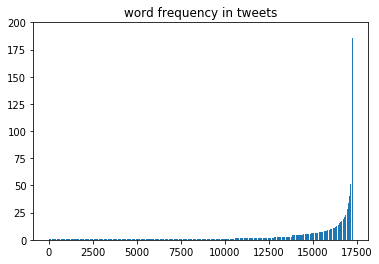
\includegraphics[scale=1]{freq}
\caption{Word frequency}
\label{freq}
\end{figure}

\section{Building models}
\subsection{Multi-Layer Perceptron (MLP)}
We tried to start with a simple model like MLP classifier, so we trained it on a word embedding-based representation of our tweets. 

For that we used the Word2Vec embeddings for our Vocabulary and represented each tweet by the sum of the embeddings of its constituents. That is, if a tweet is "Happy New Year", the value of this observation would be the sum of the embeddings of "Happy", "New" and "Year". And we do this for all the elements in the training set. Thus, using an embedding dimension of 100, the shape of our training set now becomes (number of tweets, 100).

We then trained the MLP classifier with one hidden layer of size 100 neurons, using stratified 10-fold cross-validation. We obtained the following results: 


\begin{table}[H]\centering
	\begin{tabular}{cccccccccccc}
		\toprule
		\textbf{Fold} & 0 & 1 & 2 & 3 & 4 & 5 & 6 & 7 & 8 & 9 & \textbf{Mean} \\    \midrule
		\textbf{Accuracy} & 0.513 & 0.540 & 0.513 & 0.522 & 0.5 & 0.530 & 0.521 & 0.496 & 0.487 & 0.493& \textbf{0.51}  \\   
		\bottomrule	
	\end{tabular}
	\caption{Accuracy obtained for each fold}
\end{table}

As we can see, the MLP performance is slightly better than a random classifier which would give us an accuracy of 33\% but it's not satisfying for our problem. 

\subsection{Long Short Term Memory (LSTM)}
Since the MLP classifier didn't give any good results, we decided to use recurrent neural networks which are models specialized in sequential data like the natural text in which the position of the words plays a significant role in the meaning. More precisely, we have chosen LSTM which is a robust model of the RNNs that can keep record of the long term and the short term dependencies between the parts of the data.

A common LSTM unit is composed of a cell, an input gate, an output gate and a forget gate. The cell is responsible for learning long-term dependencies through arbitrary time intervals; this allows LSTM model to handle the exploding and vanishing gradient problems that traditional RNNs suffer from. 

\subsubsection{Data matrix}

In order to train LSTM model, an input matrix must be constructed with 3 dimensions: batch size $\times$ sequence length $\times$ embeddings length, where :

\begin{itemize}
	\item Batch size = number of tweets,
	\item Sequence length = length of the longest tweet (in the train set),
	\item Embedding length : size of embeddings fixed at 100.
\end{itemize}

As we notice, tweets have different lengths. To handle this, we take the size of the longest one and use it as a reference. The tweets having the same number of words are kept as they are, and the shorter ones are duplicated until their sizes reach that of the longest tweet.

Words embeddings are calculated using $word2vec$ model which has been trained on the training set. Words from test set that don't exist in training set are replaced with the <unknown> word.

\subsubsection{Model architecture}
The architecture of our model is as following:
\begin{itemize}
	\item \textbf{LSTM layer} with a hidden state size of 200. The output of this layer is a 3 dimensional matrix in which the first 2 dimensions are as always the \emph{batch size} and the \emph{sequence length}, but the last one will be hidden state size, which is equal, in our case, to 200.
	\item \textbf{Dropout layer} with a probability of dropping equals to $0.2$ (20\% of the output of the LSTM layer is zeroed at random locations in each training iteration).
	\item \textbf{Fully connected layer} having 2 dimensions, the first one is sequence length $\times$ LSTM hidden size, and this is caused by the output of the LSTM layer which is 3 dimensional while the input of the Dropout layer is only 2 dimensional, so the last 2 dimensions of the first layer's output are flattened into a single dimension.
\end{itemize}

The optimizer used for training is \textbf{Adam}. It has been chosen instead of the simple \emph{Stochastic Gradient Descent (SGD)} since it is robust against local optima.

The loss function used is the \textbf{Cross Entropy Loss}, because we are dealing with a classification problem.

After performing the forward propagation, we backward the error gradient and update the parameters of the model. The network's memory is emptied after each iteration. The dropout layer is used as a regularization trick because it has a big impact on the model's performance. More details will be discussed later. 

\subsubsection{Implementation and Results}
We used \textbf{PyTorch} to implement our LSTM model. The program shows real-time plots for accuracy and the Cross Entropy Loss for both train and test sets.

The next figure shows the plots for the whole training process:

\begin{figure}[H]
\centering
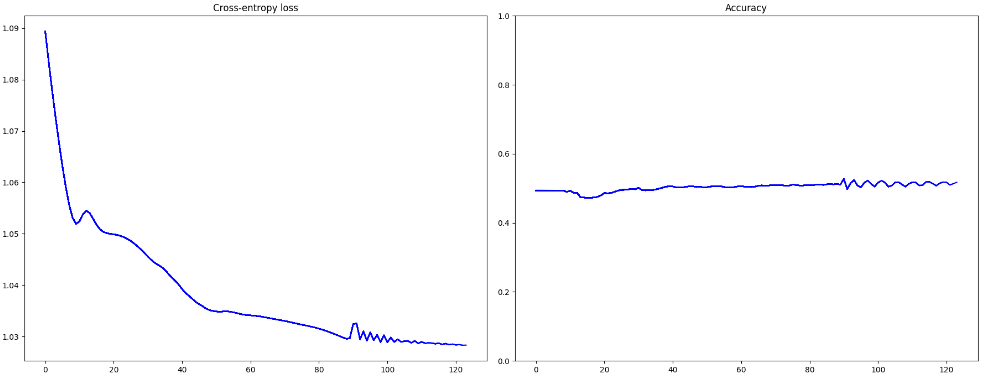
\includegraphics[width=\textwidth]{acc_loss}
\caption{Evolution of Accuracy and Cross Entropy Loss through the whole training process (Blue: Train, Green: Test)}
\end{figure}

The program also allow interrupting the training process (if under/over-fitting are observed for example or if the training process takes too long) and then saves the model's learned parameters in a file so that it will be possible to continue the learning process from where it was stopped last time.

The results of training the LSTM model after 3295 epochs (running it for 9 hours on Intel Core i5 processor) are the following:

\begin{table}[H]\centering
	\begin{tabular}{cccccccccccc}
		\toprule
		\textbf{Set} & Train & Test \\    \midrule
		\textbf{Accuracy} & 88.64\% & 89.32\% \\   
		\textbf{Cross Entropy Loss} & 0.2720 & 0.2617\\
		\bottomrule	
	\end{tabular}
	\caption{Accuracy and Cross Entropy Loss obtained with LSTM }
\end{table}


\paragraph{Why dropout layer is so important ?}
Before adding the dropout layer, the model was over-fitting the data, and the error on test set was diverging from that of training set since the first iterations ! Thus, the model was performing very well on the training data while it was very bad on the test data.

\begin{figure}[H]
	\centering
	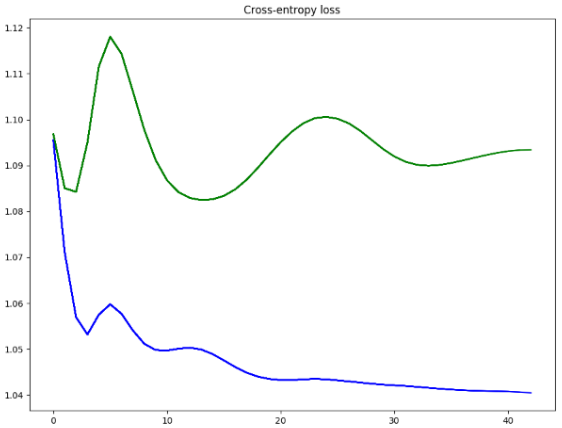
\includegraphics[scale=1]{overfitting}
	\caption{Cross Entropy Loss before adding dropout}
\end{figure}

\subsubsection{Discussion of results}
Comparing our LSTM model with the work done by Ye Yuan, You Zhou in [2], we find that their One-hidden-layer RNN has reached only \textbf{63.71\%} of accuracy on the same dataset that we used. Therefore, our LSTM model is clearly better.

We also tried the mini-batch mode but the program was very slow compared to batch mode. The latter gave us satisfying results so we decided to use it in the final version of the program.

\section{Conclusion}
In this work, we compared the performance of two neural networks: MLP and LSTM classifiers. The performance of the latter was better on tweets classification task. Therefore, LSTM is more suitable for sentiment analysis from the text thanks to its long-term memory that is not available in general models like MLP.

In addition, we found that many factors can control the efficiency of our model, especially data preprocessing quality, regularization and network architecture.

Text classification remains a large field of research and the subject of many real-world problems.

\section{References}
[1] Semeval 2013 Task 2 Data. http://www.cs.york.ac.uk/semeval-2013/task2/. Retrieved on January 4th 2018.

[2] Yuan, Y. and Zhou, Y., 2015. Twitter Sentiment Analysis with Recursive Neural Networks. CS224D Course Projects.

\end{document}
